\documentclass[tikz,border=10pt]{standalone}
% Scale: s = 0.012739 cm/px (STYLE METRICS), A at origin, y flipped
\begin{document}
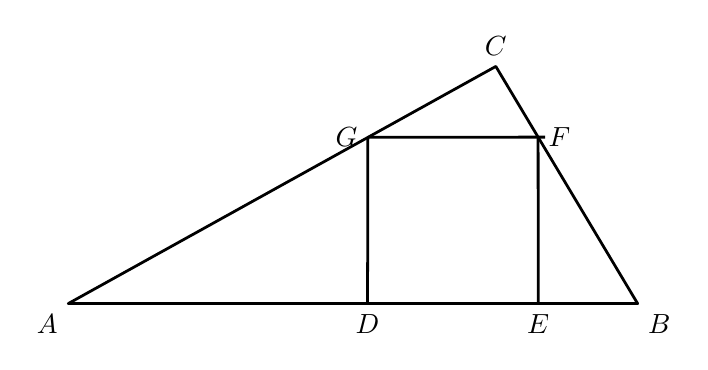
\begin{tikzpicture}[line width=1.0pt, line join=round]
  % Named coordinates (cm)
  \coordinate (A) at (0,0);
  \coordinate (B) at (7.231,0);
  \coordinate (C) at (5.430,3.012);
  \coordinate (D) at (3.801,0);
  \coordinate (E) at (5.968,0);
  \coordinate (F) at (5.967,2.114);
  \coordinate (G) at (3.805,2.113);
  % Right end of horizontal segment (x=554 px at y=148 px), unchanged
  \coordinate (H2) at (6.056,2.114);

  % Triangle ABC (solid black)
  \draw[black] (A) -- (B) -- (C) -- cycle;

  % Horizontal line from G (starts exactly at vertex G) to right end
  \draw[black] (G) -- (H2);

  % Vertical segments G-D and F-E
  \draw[black] (G) -- (D);
  \draw[black] (F) -- (E);

  % Labels in math mode with metrics font
  \node[below left, font=\fontsize{10}{12}\selectfont] at (A) {$A$};
  \node[below right, font=\fontsize{10}{12}\selectfont] at (B) {$B$};
  \node[above, font=\fontsize{10}{12}\selectfont] at (C) {$C$};
  \node[below, font=\fontsize{10}{12}\selectfont] at (D) {$D$};
  \node[below, font=\fontsize{10}{12}\selectfont] at (E) {$E$};
  \node[right, font=\fontsize{10}{12}\selectfont] at (F) {$F$};
  \node[left, font=\fontsize{10}{12}\selectfont] at (G) {$G$};
\end{tikzpicture}
\end{document}